\documentclass{standalone}
\usepackage{../preamble}

\begin{document}

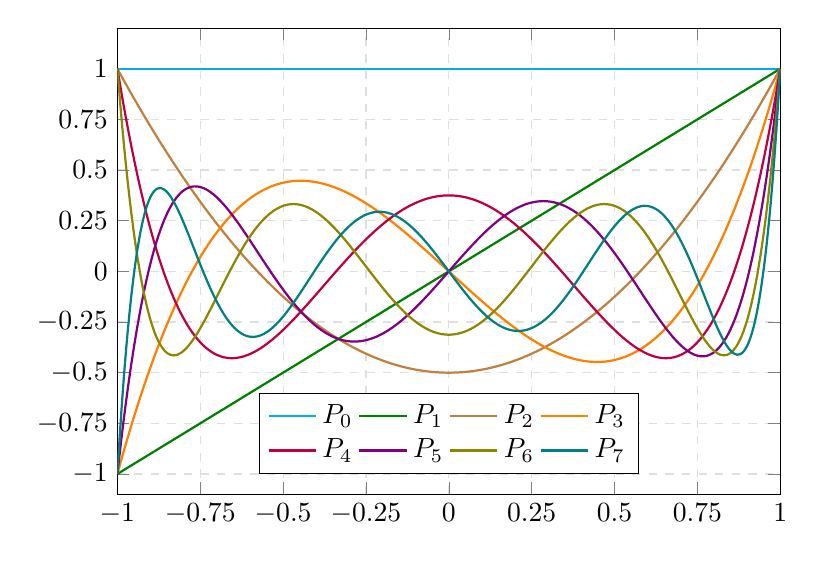
\begin{tikzpicture}
  \begin{axis}
    [
      xmin = -1, xmax = 1, %
      ymin = -1.1, ymax = 1.2, %
      xtick distance = 0.25, %Is the distance between major ticks in the x-axis.
      ytick distance = 0.25, %Is the distance between major ticks in the y-axis.
      % minor tick num = 1, %Is the number of ticks between major ticks.
      grid=major,
      major grid style = {lightgray!50, dashed}, %Changes the color and stroke of the major grid.
      minor grid style = {lightgray!25}, %Changes the color and stroke of the minor grid.
      width = 10cm, %sets the width of the figure
      height = 7.5cm,  %sets the height of the figure
      xlabel = {}, %
      ylabel = {}, %
      legend cell align = {left}, %
      legend columns=4,
      legend style={at={(axis cs:0,-0.8)},anchor=center} % position of the legend box and anchor is the point on the box to be fitted exactly at the point of cs:<>,<>. Options are anchor=center,south west,south east,north west,north east,north,south,west...
    ]
    \addplot[
      domain=-1:1, %Domain of the fucntion
      samples=200, %This parameter determines the number of point to be plotted for the function, while bigger the number better looks the function.
      smooth, %f we use this option, the compiler makes an interpolation between the point plotted to get a soft appearance for the function.
      thick, %Stroke of the function. Options: ultra thin, very thin, thin, semithick, thick, very thick, ultra thick.
      cyan %Color of the function.
    ]{1};
    \addplot[
      domain=-1:1, %Domain of the fucntion
      samples=200, %This parameter determines the number of point to be plotted for the function, while bigger the number better looks the function.
      smooth, %f we use this option, the compiler makes an interpolation between the point plotted to get a soft appearance for the function.
      thick, %Stroke of the function. Options: ultra thin, very thin, thin, semithick, thick, very thick, ultra thick.
      green!50!black %Color of the function.
    ]{x};
    \addplot[
      domain=-1:1, %Domain of the fucntion
      samples=200, %This parameter determines the number of point to be plotted for the function, while bigger the number better looks the function.
      smooth, %f we use this option, the compiler makes an interpolation between the point plotted to get a soft appearance for the function.
      thick, %Stroke of the function. Options: ultra thin, very thin, thin, semithick, thick, very thick, ultra thick.
      brown %Color of the function
    ]{1/2*(3*x^2-1)};
    \addplot[
      domain=-1:1, %Domain of the fucntion
      samples=200, %This parameter determines the number of point to be plotted for the function, while bigger the number better looks the function.
      smooth, %f we use this option, the compiler makes an interpolation between the point plotted to get a soft appearance for the function.
      thick, %Stroke of the function. Options: ultra thin, very thin, thin, semithick, thick, very thick, ultra thick.
      orange %Color of the function
    ]{1/2*(5*x^3-3*x)};
    \addplot[
      domain=-1:1, %Domain of the fucntion
      samples=200, %This parameter determines the number of point to be plotted for the function, while bigger the number better looks the function.
      smooth, %f we use this option, the compiler makes an interpolation between the point plotted to get a soft appearance for the function.
      thick, %Stroke of the function. Options: ultra thin, very thin, thin, semithick, thick, very thick, ultra thick.
      purple %Color of the function.
    ]{1/8*(35*x^4-30*x^2+3)};
    \addplot[
      domain=-1:1, %Domain of the fucntion
      samples=200, %This parameter determines the number of point to be plotted for the function, while bigger the number better looks the function.
      smooth, %f we use this option, the compiler makes an interpolation between the point plotted to get a soft appearance for the function.
      thick, %Stroke of the function. Options: ultra thin, very thin, thin, semithick, thick, very thick, ultra thick.
      violet %Color of the function
    ]{1/8*(63*x^5-70*x^3+15*x)};
    \addplot[
      domain=-1:1, %Domain of the fucntion
      samples=200, %This parameter determines the number of point to be plotted for the function, while bigger the number better looks the function.
      smooth, %f we use this option, the compiler makes an interpolation between the point plotted to get a soft appearance for the function.
      thick, %Stroke of the function. Options: ultra thin, very thin, thin, semithick, thick, very thick, ultra thick.
      olive %Color of the function
    ]{1/16*(231*x^6-315*x^4+105*x^2-5)};
    \addplot[
      domain=-1:1, %Domain of the fucntion
      samples=200, %This parameter determines the number of point to be plotted for the function, while bigger the number better looks the function.
      smooth, %f we use this option, the compiler makes an interpolation between the point plotted to get a soft appearance for the function.
      thick, %Stroke of the function. Options: ultra thin, very thin, thin, semithick, thick, very thick, ultra thick.
      teal %Color of the function
    ]{1/16*(429*x^7-693*x^5+315*x^3-35*x)};
    \legend{$P_0$,$P_1$,$P_2$,$P_3$,$P_4$,$P_5$,$P_6$, $P_7$}

    % Legendre polynomials:
    % p_0(x) = 1
    % p_1(x) = x
    % p_2(x) = 1/2*(3*x^2-1)
    % p_3(x) = 1/2*(5*x^3-3*x)
    % p_4(x) = 1/8*(35*x^4-30*x^2+3)
    % p_5(x) = 1/8*(63*x^5-70*x^3+15*x)
    % p_6(x) = 1/16*(231*x^6-315*x^4+105*x^2-5)
    % p_7(x) = 1/16*(429*x^7-693*x^5+315*x^3-35*x)
    % p_8(x) = 1/128*(6435*x^8-12012*x^6+6930*x^4-1260*x^2+35)
  \end{axis}
\end{tikzpicture}
\end{document}